\documentclass{standalone}
\usepackage{tikz}
\usetikzlibrary{calc,positioning,shapes,decorations.pathmorphing}
\usetikzlibrary{hobby} % for blobs, see http://tex.stackexchange.com/a/145276

\def\gridopacity{100}
\def\gridopacity{0}

\begin{document}%
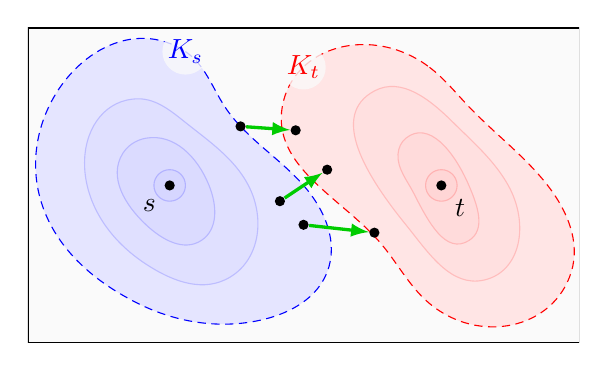
\begin{tikzpicture}

\tikzset{>=latex} % arrow heads

\draw[step=1,black!15,very thin,opacity=\gridopacity] (0,0) grid (5,4);

\begin{scope}
\clip (0,0) rectangle (7,4);
\fill[black!2] (0,0) rectangle (7,4);


% draw some contour blobs

% start side
%\path[draw,use Hobby shortcut,closed=true,fill=black!2,draw=black!16]
%   (4.9,4.0) .. (4.6,3.0) .. (5.4,2.0) .. (5.6,1.0) .. (5.9,0) .. (-0.6,-1.1);
%\path[draw,use Hobby shortcut,closed=true,fill=black!4,draw=black!18]
%   (4.0,4.0) .. (3.9,3.0) .. (4.9,2.0) .. (5.1,1.0) .. (5.4,0) .. (-0.1,-0.6);
%\path[draw,use Hobby shortcut,closed=true,fill=black!6,draw=black!20]
%   (2.9,3.9) .. (3.2,3.0) .. (4.1,2.0) .. (4.5,1.0) .. (4.4,0) .. (0.4,0.0);
\path[draw,use Hobby shortcut,closed=true,fill=blue!10,densely dashed,draw=blue]
   (2.0,3.7) .. (2.5,3.0) .. (3.5,2.0) .. (3.8,0.9) .. (3.0,0.3) .. (1.4,0.5);
\path[draw,use Hobby shortcut,closed=true,fill=blue!12,draw=blue!26]
   (1.4,3.1) .. (2.0,2.8) .. (2.8,2.0) .. (2.5,0.8) .. (1.5,1.0);
\path[draw,use Hobby shortcut,closed=true,fill=blue!14,draw=blue!28]
   (1.2,2.4) .. (1.5,2.6) .. (2.3,2.0) .. (2.2,1.3) .. (1.5,1.5);
\path[draw,use Hobby shortcut,closed=true,fill=blue!16,draw=blue!30]
   (2.0,2.0) .. (1.8,2.2) .. (1.6,2.0) .. (1.8,1.8);

% goal side
%\path[draw,use Hobby shortcut,closed=true,fill=black!6,draw=black!20]
%   (5.0,4.0) .. (6.8,2.6) .. (7.3,0.4) .. (5.0,0.0) .. (4.25,0.8) .. (2.7,3.0);
\path[draw,use Hobby shortcut,closed=true,fill=red!10,densely dashed,draw=red]
   (5.1,3.5) .. (5.6,3.0) .. (6.6,2.0) .. (6.9,0.9) .. (5.1,0.5) .. (4.45,1.3) .. (3.23,3.0);
\path[draw,use Hobby shortcut,closed=true,fill=red!12,draw=red!26]
   (4.4,3.2) .. (5.4,2.8) .. (6.1,2.0) .. (5.8,0.8) .. (4.8,1.5);
\path[draw,use Hobby shortcut,closed=true,fill=red!14,draw=red!28]
   (4.7,2.4) .. (4.8,2.6) .. (5.6,2.0) .. (5.6,1.3) .. (4.9,1.9);
\path[draw,use Hobby shortcut,closed=true,fill=red!16,draw=red!30]
   (5.45,2.0) .. (5.25,2.2) .. (5.05,2.0) .. (5.25,1.8);

\node[circle,fill=black!2,fill opacity=0.8,text opacity=1.0,inner sep=0.5pt,text=blue] at (2.0,3.7) {$K_s$};
\node[circle,fill=black!2,fill opacity=0.8,text opacity=1.0,inner sep=0.5pt,text=red] at (3.5,3.5) {$K_t$};


%\draw[step=1,black!30,very thin,opacity=0.5] (0,0) grid (7,4);
\draw (0,0) rectangle (7,4);
\end{scope}

% vertices
\node[fill=black,circle,inner sep=1.3pt] (s) at (1.8,2.0) {};
\node[below left=0.0cm of s] {$s$};
\node[fill=black,circle,inner sep=1.3pt] (t) at (5.25,2.0) {};
\node[below right=0.0cm of t] {$t$};

% one edge
\node[fill=black,circle,inner sep=1.3pt] (a1) at (3.2,1.8) {}; % frontier
\node[fill=black,circle,inner sep=1.3pt] (a2) at (3.8,2.2) {}; % frontier
\draw[->,draw=green!80!black,very thick] (a1) -- (a2);

% above edge
\node[fill=black,circle,inner sep=1.3pt] (b1) at (2.7,2.75) {}; % frontier
\node[fill=black,circle,inner sep=1.3pt] (b2) at (3.4,2.7) {}; % frontier
\draw[->,draw=green!80!black,very thick] (b1) -- (b2);

% below edge
\node[fill=black,circle,inner sep=1.3pt] (c1) at (3.5,1.5) {}; % frontier
\node[fill=black,circle,inner sep=1.3pt] (c2) at (4.4,1.4) {}; % frontier
\draw[->,draw=green!80!black,very thick] (c1) -- (c2);


\end{tikzpicture}%
\end{document}
